\documentclass[11pt]{article}

\usepackage[utf8]{inputenc}
\usepackage{listings}
\usepackage{color}
\usepackage{graphicx}

% \usepackage[ngerman]{babel}
\setlength{\textwidth}{5.5in}

\title{Corba Übung}
\author{Nikolaus Schrack, Gary Ye (4BHIT)}
\date{\today{}, Wien}
\begin{document}

\maketitle

\tableofcontents
\newpage

\lstset{basicstyle=\ttfamily\small,
        keywordstyle=,
        commentstyle=\itshape,
        numbers=left,                   % where to put the line-numbers
        stepnumber=1,
        breaklines=true,					% line wrapping on
        numberstyle=\tiny,
        showstringspaces=false,
        abovecaptionskip=0pt,
        belowcaptionskip=0pt,
        xleftmargin=\parindent,
        fontadjust}

\section{Aufgabenstellung}
Verwenden Sie das Paket ORBacus oder omniORB bzw. JacORB um Java und C++ ORB-Implementationen zum Laufen zu bringen.

Passen Sie eines der Demoprogramme so an, dass Sie einen Namingservice verwenden, welches ein Objekt anbietet, das von jeweils einer anderen Sprache (Java/C++) verteilt angesprochen wird. Beachten Sie dabei, dass eine IDL-Implementierung vorhanden ist um die unterschiedlichen Sprachen abgleichen zu können.

Vorschlag: Verwenden Sie für die Implementierungsumgebung eine Linux-Distribution, da eine optionale Kompilierung einfacher zu konfigurieren ist.

\subsection{Resources}

\begin{itemize}
\item http://omniorb.sourceforge.net/
\item http://www.microfocus.com/products/corba/orbacus/
\item http://www.jacorb.org/
\item http://omniorb.sourceforge.net/omni41/omniORB.pdf
\item http://www.ing.iac.es/~docs/external/corba/book.pdf
\end{itemize}

\section{Aufwandsschätzung}
\subsection{Geschätzter Aufwand}

\begin{center}
  \begin{tabular}{| l | l | l |}
    \hline
    Task & Schrack & Ye \\ \hline

    Dokumentierung des C++ Servers   & 0h & \\ \hline
    Dokumentierung des Java Clients  & & 6h \\ \hline
    Implementierung des Java Clients & & 4h \\ \hline
  \end{tabular}
\end{center}

\subsection{Tatsächlicher Aufwand}
\begin{center}
  \begin{tabular}{| l | l | l |}
    \hline
    Task & Schrack & Ye \\ \hline
    Dokumentation Allgemein          & 0h & h \\ \hline
    Dokumentierung des C++ Servers   & 0h & \\ \hline
    Dokumentierung des Java Clients  & & 2h \\ \hline
    Implementierung des Java Clients & & 2h \\ \hline
  \end{tabular}
\end{center}

Weil wenig Erfahrung in dem Gebiet besteht, wurde eine sehr hohe Aufwandszeit geschätzt. Die Zeit wurde hauptsächlich mit dem Lesen der beiliegenden Dokumentationen verbracht, damit das Implementieren ohne Zweifeln ausgeführt werden konnte.

\section{Designüberlegung}
Da beide Teammitglieder Corba-Neulinge sind, wurde aus Erfahrung beschlossen, dass das Lesen der Dokumentationen der beste Start in eine neue Übung bzw. Aufgabe ist. Nachher sind die neue Technologien und der Quellcode, der beiliegenden Beispiele, einigermaßen klarer geworden. Im omniORB-Verzeichnis gibt es ein ``echo-example'', das eine in C++ implementierte Version von Server und Client, die den NamingService verwenden, enthält. Danach wurde ausgemacht, dass Gary Ye die Java Client Version schreibt und seine Vorgänge niederschreibt, und dass Nikolaus Schrack den größten Teil des C++ Source Codes dokumentiert. 

\section{Installation}

\subsection{OmniORB}

Die folgende Packages werden für die Installation von OmniORB benötigt: omniorb omniorb-doc omniorb-idl omniorb-nameserver python2.7-dev. Diese sollten entsprechend mit apt-get installiert werden und danach ladet man die Installationsdateien von der offiziellen OmniORB Seite [1] runter (es wurde für die Übung omniORB-4.1.7 benutzt). Anschließend wechselt man in den Omniorb Directory und führt die folgende Befehle, die auch im Readme erwähnt sind, aus.

\begin{lstlisting}
mkdir build
cd build
../configure
make
make install
\end{lstlisting}

Man kann auch den Installationsort ändern, indem man einen Wert für --prefix angibt. Sollte man keinen angeben, so werden sie per Default im /usr/local Verzeichnis installiert.

\begin{lstlisting}
../configure --prefix=/home/gary/omni_inst
\end{lstlisting}

\subsection{JacORB}

\begin{lstlisting}
wget http://www.jacorb.org/releases/3.2/jacorb-3.2-source.zip
unzip jacorb-3.2-source.zip
ant all
\end{lstlisting}

\section{Implementierung}

\subsection{IDL File}

IDL (Interface Definition Language) ist eine deskriptive Sprache zum Beschreiben der Interfaces in einem Softwareprogramm. Das Beschreiben geschieht Programmiersprache-unabhängig, damit Softwarekomponenten, die in verschiedenen Programmiersprachen geschrieben wurden (wie z.B. C++, Java, Python), miteinander kommunizieren können. Man kann das IDL File mit Hilfe eines IDL Compilers zu einem sprachspezfischen Quellcode kompillieren (z.B. Stubs, Skeletons, etc.). 

Der folgende Code ist von das am ``Echo'' Inteface angepasste IDL File(echo.idl). Anzumerken ist, dass es einen Modul namens ``schrackye'' existiert. Module sind ähnlich wie Packages von Java oder Namespaces von C++. 

\lstset{language=IDL}  

\begin{lstlisting}
#ifndef __ECHO_IDL__
#define __ECHO_IDL__
module schrackye {
        interface Echo {
                string echoString(in string mesg);
        };
};
#endif // __ECHO_IDL__         

\end{lstlisting}

\begin{description}
\item[Line 1-2, 8] \hfill \\
\#ifndef \_\_ECHO\_IDL sind wie man von C kennt Header Guards, die vor Doppeldeklarationen schützen sollen. 
\item[Line 3] \hfill \\
Man definiert Module wie Namespaces in C++. Man sollte beachten, dass, dass ein Semikolon ``;'' hinter der geschlossenen geschwungenen Klammer ``\}'' gehört.
\item[Line 4] \hfill \\
Die Deklaration von Interfaces kennt man von Java, auch hier muss man am Ende ein Semikolon schreiben.
\item[Line 5] \hfill \\


\end{description}
Um den Java Stub Code zu generieren führt man den folgenden Befehl aus:

\lstset{language=bash}
\begin{lstlisting}
idlj echo.idl
\end{lstlisting}
Oder für C++
\begin{lstlisting}
omniidl echo.idl
\end{lstlisting}

\subsection{C++ Server}

Der größte Teil vom Code wurde vom Echo Example entnommen. Es werden die essenziellen Teile Teile des Codes beschrieben. 

In dem folgenden Codesnippet wird das Echo Interface implementiert.

\begin{lstlisting}
class Echo_i : public POA_schrackye::Echo
{
public:
  inline Echo_i() {}
  virtual ~Echo_i() {}
  virtual char* echoString(const char* mesg);
};


char* Echo_i::echoString(const char* mesg)
{
  return CORBA::string_dup(mesg);
}
\end{lstlisting}



Zunächst wird die main Methde geschrieben

\begin{lstlisting}
CORBA::ORB_var orb = CORBA::ORB_init(argc, argv);

CORBA::Object_var obj = orb->resolve_initial_references("RootPOA");
PortableServer::POA_var poa = PortableServer::POA::_narrow(obj);

Echo_i* myecho = new Echo_i();

PortableServer::ObjectId_var myechoid = poa->activate_object(myecho);

obj = myecho->_this();

CORBA::String_var x;
x = orb->object_to_string(obj);
cout << x << endl;

if( !bindObjectToName(orb, obj) )
	return 1;

myecho->_remove_ref();

PortableServer::POAManager_var pman = poa->the_POAManager();
pman->activate();

orb->run();
\end{lstlisting}

\begin{description}

\item[Line 1] \hfill \\
Hier wird der ORB mit den Kommandozeilenargumenten initialisiert.

\item[Line 3-4] \hfill \\
Der Server wird für die Client sichtbar gemacht. Dies wird mit der Registrierung bei der POV, in unserem fall das \textit{Root POA} durchgeführt.

\item[Line 6] \hfill \\
Eine Instanz von Echo wird erstellt.

\item[Line 9] \hfill \\
\end{description}

\subsection{Java Client}

Der folgende Java Code führt einen Remote Procedure Call (RPC) aus, um eine Nachricht, die man an den Server übergibt, von ihm wieder zurückbekommt (also im Prinzip der Aufruf der Methode echoString).

\begin{lstlisting}
package schrackye;

import java.util.Properties;

import org.omg.CosNaming.*;
import org.omg.CosNaming.NamingContextPackage.InvalidName;

public class Client {
    public static void main(String[] args){
	Echo echo;
	try{
	    org.omg.CORBA.ORB orb = org.omg.CORBA.ORB.init(args, null);

	    org.omg.CORBA.Object o = orb.resolve_initial_references("NameService");
	    NamingContextExt rootContext = NamingContextExtHelper.narrow( o );
			
	    NameComponent[] name = new NameComponent[2];
	    name[0] = new NameComponent("test","my_context");
	    name[1] = new NameComponent("Echo", "Object");
		
	    echo = EchoHelper.narrow(rootContext.resolve(name));
	    System.out.println("Server says : " + echo.echoString("Juhu funktioniert!"));
	} catch(InvalidName e){
	    System.err.println("InvalidNameException occured : " + e.getMessage());
	} catch(Exception e){
	    System.err.println("Unknown exception occured : " + e.getMessage());
	    e.printStackTrace();
	}
    }
}
\end{lstlisting}

\begin{description}
\item[Line 12] \hfill \\
Hier initialisiert man den ORB. Man übergibt ih die Programmargumente ``args'' von der Kommandozeile und er bearbeitet alle die den Präfix ``-ORB'' besitzen. Die Kommandoargumente ist eine Alternative zu dem Property File.

\item[Line 14-15] \hfill \\
Hier erhält man den RootContext des angegebenen Namingservices. 

\item[Line 17-19] \hfill \\
% TODO id, kind?

\item[Line 21] \hfill \\
Hier wird der Name, den wir angegeben haben aufgelöst. Da die Methode``resolve()'' ein Objekt vom Typ org.omg.CORBA.Object zurückgibt, muss man mit Hilfe von dem entsprechenden Helper, die Rückgabe in den Ursprungstyp zurückformen lassen.

\item[Line 22] \hfill \\
Die Methode wird mit Hilfe von einem RPC aufgerufen und das Ergebnis lässt sich dann im Output sehen.

\end{description}

\section{Ausführung}

\section{Aufgetretene Probleme}

\section{Testbericht}

\subsection{Lokales Testing}

Anfangs wurde nur lokal getestet, d.h. Server und Client sind beide auf der selben Maschine gewesen. Er ist wie auf dem Bild zu sehen, erfolgreich abgelaufen. Das linke Terminal ist eine Debian VirtualMachine (mit SSH verbunden), während auf der rechten Seite eine Ubuntu Maschine läuft.
% trim=1cm 2cm 3cm 4cm, clip=true, totalheight=0.5\textheight, angle=90]
% left bottom right top

\begin{center}
  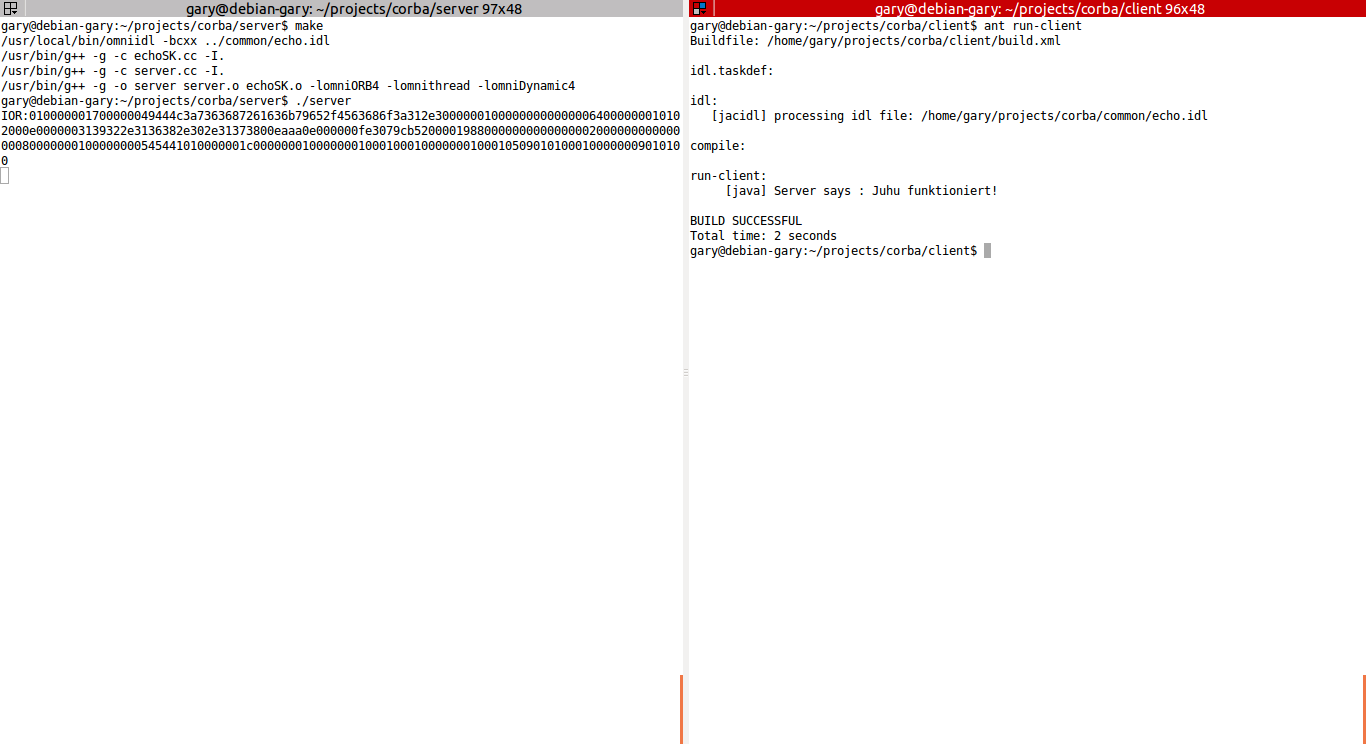
\includegraphics[width=\linewidth, height=1in]{test_local}
\end{center}
\subsection{Testing über das Netzwerk}

Noch ein Bild von dem Testen über das Netzwerk, das erfolgreich abgelaufen ist.
\begin{center}
  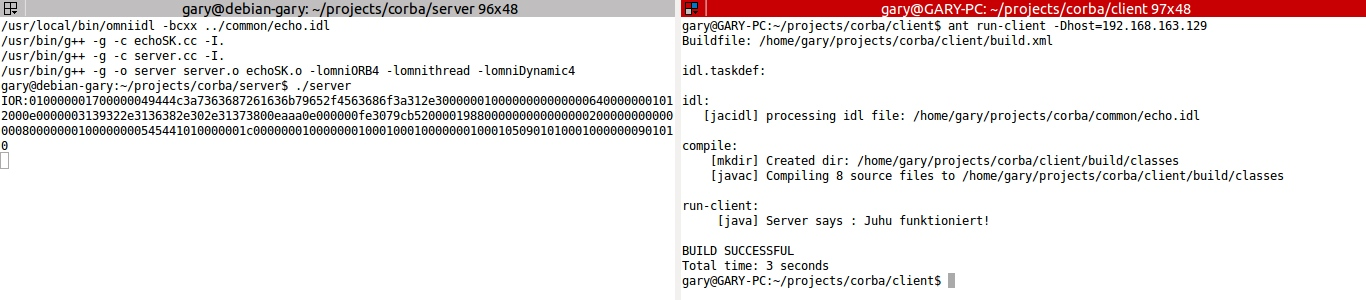
\includegraphics[width=\linewidth, height=1in]{test_network}
\end{center}

\section{Quellen}

\bibliography{references}{}
\bibliographystyle{plain}

% \printbibliography
\end{document}
